%
% main.tex -- Paper zum Thema verzoegerte Differentialgleichung
%
% (c) 2018 Raphael Unterer, Hochschule Rapperswil
%
\chapter{Numerische Lösung einer verzögerten Differentialgleichung\label{chapter:verzoegert}}
\lhead{Numerische Lösung einer verzögerten Differentialgleichung}
\begin{refsection}
\chapterauthor{Raphael Unterer}

\section{Einleitung}
Verzögerte Differentialgleichungen sind gewöhnliche Differentialgleichungen, bei welchen die Ableitung von früheren Funktionswerten abhängt.
Ein gutes Beispiel dafür ist die Populationsentwicklung in der Biologie. 
Für das Populationswachstum bei Tieren ist entscheidend wie viele junge Tiere geschlechtsreif werden.
Somit hängt das Wachstum von einem früheren Wachstum ab, da es einige Zeit dauert bis die Jungen geschlechtsreif sind.
Es gibt diverse weitere Anwendungen für verzögerte Differentialgleichungen in Physik, Chemie und Biologie (vgl. \cite{verzoegert:erneux}).

Hier wollen wir vor allem die verzögerte Differentialgleichung zur Modellierung des El Niño Phänomens  betrachten. %todo ev. Verweis?
Wir lernen zuerst einige grundlegende Methoden kennen, um eine verzögerte Differentialgleichung analytisch zu untersuchen. 
Danach wird gezeigt, wie eine numerische Berechnung gemacht wird.

%
% main.tex -- Paper zum Thema verzoegerte Differentialgleichung
%
% (c) 2018 Raphael Unterer, Hochschule Rapperswil
%
\section{Grundlagen verzögerte Differentialgleichungen}
\rhead{Grundlagen DDE}
\subsection{Definitionen}
Verzögerte Differentialgleichungen werden als DDE (engl. "\textbf{D}elayed \textbf{D}ifferential \textbf{E}quation") abgekürzt.

Die allgemeine DDE 1. Ordnung sieht folgendermaßen aus:
\begin{equation}
	\dot{x}(t) = f(x(t),x(t-\tau_1),...,x(t-\tau_n))
\end{equation}
Dabei ist $f$ eine beliebige Funktion. Die Verzögerungen $\tau_1,...,\tau_n$ sind gegeben und nach der Grösse geordnet, also $0<\tau_1<...<\tau_n$.

Im Unterschied zu einer gewöhnliche Differentialgleichung ist das Anfangswertproblem nicht mehr eindimensional, d.h. es genügt nicht mehr den Anfangszustand zu kennen.
Alle Werte von $-\tau_n$ bis $0$ müssen gegeben sein. 
Es braucht somit eine unendliche Anzahl Anfangswertvektoren, welche bekannt sein müssen.

In den folgenden Betrachtungen analysieren wir die einfachste DDE:
\begin{equation}\label{bsp}
\dot{y}(t)=ky(t-\tau)
\end{equation}

\subsection{Schrittweises Lösen}
Beim schrittweisen wird die DDE immer in Schritten von einem $\tau$ gelöst.
Wir nehmen an, dass $y$ im Bereich von $-\tau$ bis $0$ immer Konstant bleibt
\begin{equation}
	y(t)=1 \text{ wenn } -1\le t<0
\end{equation}
Daraus folgt, dass im Bereich von $0\le t<\tau$ die Ableitung
\begin{equation}\label{abl}
	\dot{y}(t)=k
\end{equation}
wird. Durch integrieren von \ref{abl} erhalten wir
\begin{equation}
	y(t)=1+kt
\end{equation}
für den Bereich $0\le t<\tau$. 
Dieses $y(t)$ kann als Anfangswert für den nächsten Schritt genommen werden.
Wir erhalten für den zweiten Schritt  $\tau\le t<2\tau$ 
\begin{equation}\label{abl2}
	\dot{y}(t)=k(1+k(t-\tau))=k+k^2(t-\tau)
\end{equation}
Es ist offensichtlich das diese Methode nur für kurze Zeiten, einfache Anfangswerte und einfache Formeln funktioniert. 
Bereits \ref{abl2} ist nicht mehr ganz einfach zu Integrieren. 
Für längere Zeiten werden die Integrale immer komplexer. %todo ev simulation matlab

\subsection{Charakteristisches Polynom}
Bei gewöhnlichen Differentialgleichungen können Lösungen mit Hilfe des charakteristischen Polynoms gefunden werden. 
Bei DDEs wird das Polynom zu einer Gleichung. 
Wir betrachten wiederum die Gleichung \ref{bsp} und verwenden als Lösungsansatz
\begin{equation}\label{ansatz}
	y(t) = ce^{\lambda t}
\end{equation}
Dieser klassische Ansatz eignet sich (fast) immer, da die Exponentialfunktion beim differenzieren erhalten bleibt. 
\ref{ansatz} eingesetzt in \ref{bsp} ergibt
\begin{equation}
	\lambda ce^{\lambda t} = kce^{\lambda (t-\tau )}
\end{equation} 
Diese Gleichung kann gekürzt werden zu
\begin{equation}
\lambda  - ke^{-\lambda \tau}= 0
\end{equation} 
Damit können nun verschiedene Werte für die Konstante $k$ berechnet werden, je nachdem wie Lösung aussehen soll. 
Die charakteristische Gleichung ist somit  eine Hilfe um Konstanten zu bestimmen, falls eine bestimmte Lösung erreicht werden soll.
\section{El Niño DDE}
\rhead{El Niño DDE}


\subsection{Gleichung}
Zur Modellierung des El Niño Effektes wurde die folgende DDE gefunden %todo Verweis Gleichung El Niño
\begin{equation} \label{eldde}
\dot{T}(t)=-cT(t)+aT(t-\frac{1}{2}\tau_K)-bT(t-(\frac{1}{2}\tau_R+\tau_K))-\epsilon(T(t))^3
\end{equation}
Mit dieser DDE wird die Änderung der Meerestemperatur $T$ vor der Küste Südamerikas beschrieben.
Die Konstanten $c,a,b,\epsilon$ müssen so bestimmt werden, dass die DDE ein möglichst gutes Resultat ergibt.
Erst wenn diese Konstanten grob bestimmt sind, kann eine sinnvolle numerische Simulation gestartet werden.
Hilfreich sind vor allem ungefähre Verhältnisse zwischen den Konstanten, so dass man zumindest einen Anhaltspunkt für die Simulation hat.
Die Verzögerungen $\tau_K$ und $\tau_R$ sind ungefähr bekannt aus physikalischen Untersuchungen der Rossby- und Kelvinwellen.
\begin{equation}
	\tau_K \approxeq \frac{1}{6}yr \text{ und } \tau_R \approxeq \frac{4}{6}yr
\end{equation}
Die Konstante $\epsilon$ ist nur zur Stabilisation, d.h. wir wählen diese so klein wie möglich.


\subsection{Charakteristische Gleichung}
Die charakteristische Gleichung für die DDE \ref{eldde} scheint sehr schwierig zu sein. 
Aus diesem Grund vereinfachen wir die DDE so weit, bis wir einen Ansatz versuchen können.
Als erstes Linearisieren wir die DDE und erhalten
\begin{equation}
	\dot{T}(t)=-cT(t)+aT(t-\frac{1}{2}\tau_K)-bT(t-(\frac{1}{2}\tau_R+\tau_K))
\end{equation}
Als nächsten Schritt setzen wir $\tau_K=0$ \footnote{$\tau_K=0$ weil $\tau_K << \tau_R$}und erhalten
\begin{equation}
	\dot{T}(t)=-cT(t)+aT(t)-bT(t-(\frac{1}{2}\tau_R))
\end{equation}
Nun stellen wir eine einfache DDE auf mit $\alpha = a-c$, $\beta = b$ und $\tau = \frac{1}{2}\tau_R$.
\begin{equation}
	\dot{T}(t)=\alpha T(t)-\beta T(t-\tau)
\end{equation}
In diese DDE setzen wir nun den bekannten Ansatz $e^{-\lambda t}$ mit $\lambda \in \mathbb{C}$ ein und erhalten
\begin{equation}
	\lambda e^{\lambda t} = \alpha e^{\lambda t} - \beta e^{\lambda(t-\tau)} \Longrightarrow \lambda = \alpha-\beta e^{-\lambda \tau}
\end{equation}
Es ist offensichtlich das beliebig viele Lösungen für Lambda möglich sind.
Da das El Niño Phänomen oszilliert, betrachten nur die Lösungen wo $\lambda$ rein imaginär wird. 

\subsection{Zusammenfassung der Analytischen Betrachtungen}
\section{Numerische Lösung}
\rhead{Numerische Lösung}

Die El-Niño-DDE soll mithilfe von Matlab numerisch gelöst werden.
Matlab stellt zum Lösen von DDEs eine fertige Funktion zu Verfügung (dde23).
Da diese Funktion auf anderen Systemen (z.B. Octave) nicht verwendbar ist, soll eine eigene Lösungsfunktion geschrieben werden.
Beim Schreiben dieser Funktion wird darauf geachtet, dass die Syntax mit dde23 vergleichbar ist. 

Es werden zwei verschiedene Ansätze implementiert: 
\begin{itemize}
	\item Berechnung von endlich kurzen Zeitschritten
	\item Berechnung über die Laplacetransformation
\end{itemize}

\subsection{Analyse der Funktion dde23}
Die offizielle Syntax von dde23 \footnote{https://www.mathworks.com/help/matlab/ref/dde23.html} lautet: 
\begin{lstlisting}{dde23}
	sol = dde23(ddefun,lags,history,tspan);
\end{lstlisting}
Wir analysieren zunächst alle Parameter.

\subsubsection{Parameter: ddefun}
Die ddefun stellt die eigentliche DDE dar, welche als Funktion übergeben werden muss.
Unsere El-Niño-DDE \ref{eldde} hat als eigene Parameter die Zeit (t), den aktuellen Wert (y), die verzögerten Werte (Z) und alle Konstanten.
\begin{lstlisting}{dde_full}
	function dydt = dde_full(t,y,Z,c,a,b,e)
	ylag1 = Z(:,1);
	ylag2 = Z(:,2);
	dydt = -c*y+a*ylag1-b*ylag2-e*y.^3;
\end{lstlisting}
Damit diese Funktion akzeptiert wird, müssen die Konstanten gesetzt werden.
\begin{lstlisting}{my_dde}
	c = 1; a = 2.6; b = 3; e = 0.1;
	my_dde = @(t,y,Z) dde_full(t,y,Z,c,a,b,e);
\end{lstlisting}

\subsubsection{Parameter: lags}
Die Verzögerungen (in Jahren) entsprechen einem simplen Vektor.
\begin{lstlisting}{lags}
	tauk = 0.15; taur = 1;
	tau = [0.5*tauk 0.5*taur+tauk];
\end{lstlisting}

\subsubsection{Parameter: history}
Die history entspricht einer Funktion, welche die Werte aus der Vergangenheit ausgibt. 
Das kann mit Vektoren (mit realen Daten\footnote{http://www.cpc.ncep.noaa.gov/data/indices/sstoi.indices}) und einer Interpolation gelöst werden.
\begin{lstlisting}{hist}
	function s = dde_hist(t)
	t_v = [-0.67,-0.58,-0.5,-0.42, ...];
	s_v = [0.71,0.5,-0.06,-0.4,...];  
	s = @(t) interp1(t_v,s_v,t);
\end{lstlisting}

\subsubsection{Gesamte Anwendung}
Der Parameter tspan gibt die zu berechnende Zeitspanne (hier 0-3 Jahre) an.
\begin{lstlisting}{Anwendung}
	sol = dde23(my_dde,tau,dde_hist,[0, 3]);
\end{lstlisting}
Der Aufruf dde23 soll nun durch eine eigene Funktion ersetzt werden.
 

\subsection{Berchnung von endlich kurzen Zeitschritten}
Bei diesem Ansatz wird immer die Ableitung zu einer bestimmten Zeit berechnet.
Diese Ableitung wird dann für einen (kurzen) Zeitschritt als Konstant genommen und damit nächste Wert berechnet.
\begin{algorithm}
	\caption{Numerischer DDE-Solver}
	\label{algo1}
	\begin{algorithmic}[1]
		\State Initialisieren, d.h. Zeitachse erstellen, Zeitschritt dt berechnen, etc
		\For{dt in t}
		\State Bestimmen ob die verzögerten Werte dde\_hist oder in alter Lösung (wenn t > $\tau$) vorkommen
		\For{i in tau}
		\State Korrekten verzögerten Wert für jedes $\tau$ finden
		\EndFor
		\State dde-Funktion aufrufen und dydt speichern
		\State Nächster Wert = aktueller Wert + dydt*dt
		\EndFor
	\end{algorithmic}
\end{algorithm}

Mit diesem Algorithmus wird ein identisches Ergebnis wie mit dde23 erreicht. 
Es werden jeweils 10000 Datenpunkte berechnet. 
Bei mehr Datenpunkten dauert die Berechnung sehr lange, wohl auch weil der Algorithmus nicht optimiert ist.
Bei dde23 werden keine fixen Zeitschritte dt berechnet, sondern eine Abschätzung des Fehlers wird vorgenommen.
Falls der geschätzte Fehler hoch ist, wird ein kleiner Zeitschritt berechnet. 
Bei kleinem Fehler (z.B. Sinus-Maximum) werden entsprechend große Zeitschritte gerechnet. %todo add Grafik


\subsection{Laplacetransformation}
Die Laplacetransformation beschreibt eine Transformation vom Zeit zum (komplexen) Frequenzbereich.
Diese Transformation ist folgendermaßen definiert:
\begin{equation}
	F(s)=\int_{0}^{\infty}f(t)e^{-st}dt \text{ wobei } s=j\omega
\end{equation} 
Für die Laplacetransformation gibt es einige bekannte Eigenschaften. 
Eine davon ist die Verschiebung im Zeitbereich, eine Andere die Ableitung.
\begin{align}
	f(t-t_0)\: \laplace \: F(s)e^{-t_0 s}\\
	\frac{\partial f(t)}{\partial t}\: \laplace \: sF(s)-f(0^+)
\end{align}
Mit dieser Eigenschaft können wir nun unsere DDE \ref{eldde} Transformieren.
Wir verwenden für die Laplacetransformierte der Temperatur $T$ das Formelzeichen $F$.
Da es keine Regeln für den kubischen Term gibt, wir $\epsilon = 0$ gesetzt.
\begin{align}
	T(t)\: \laplace \: F(s)\\
	sF(s)-T(0^+)=-cF(s)+aF(s)e^{-\frac{1}{2}\tau_K s}-bF(s)e^{-(\frac{1}{2}\tau_R + \tau_K) s}
\end{align}
Diese Gleichung können wir nach $F(s)$ auflösen und erhalten:
\begin{equation}
	F(s) = \frac{T(0)}{s+c-ae^{-\frac{1}{2}\tau_K s}+be^{-(\frac{1}{2}\tau_R + \tau_K)s}}
\end{equation}
%todo Erklären wieso es nicht funktioniert

\section{Auswertung}
\rhead{Auswertung}
\subsection{Simulation El-Niño mit realen Werten}
Der Matlab-Code zur Simulation des El-Niño DDE ist nun vorhanden.
Damit die Simulation sinnvoll ist, wird eine Zeitperiode in der Vergangenheit berechnet.
Ausgewählt zur Simulation wird die Zeitperiode ab September 1995. 
Also werden die Daten von Januar bis September 1995 als History genommen.

Simuliert werden 1 Jahr (Abbildung \ref{fig:sim1}), 3 Jahre (Abbildung \ref{fig:sim3}) und 10 Jahre (Abbildung \ref{fig:sim10}). 
Die Konstanten wurden so verändert, dass das Resultat auf 3 Jahre gut stimmt.
\begin{figure}
	\centering
	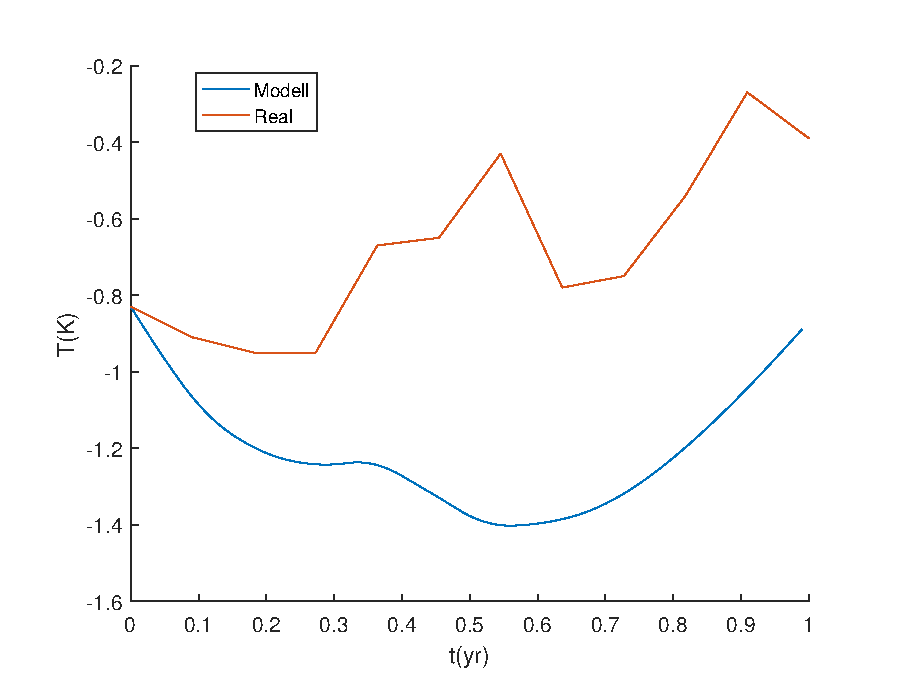
\includegraphics[width=0.66\textwidth,height=0.33\textheight]{verzoegert/inp/figures/sim_1.eps}
	\caption{El-Niño Simulation von 1995-1996 und Vergleich mit realen Daten}
	\label{fig:sim1}
\end{figure}
\begin{figure}
	\centering
	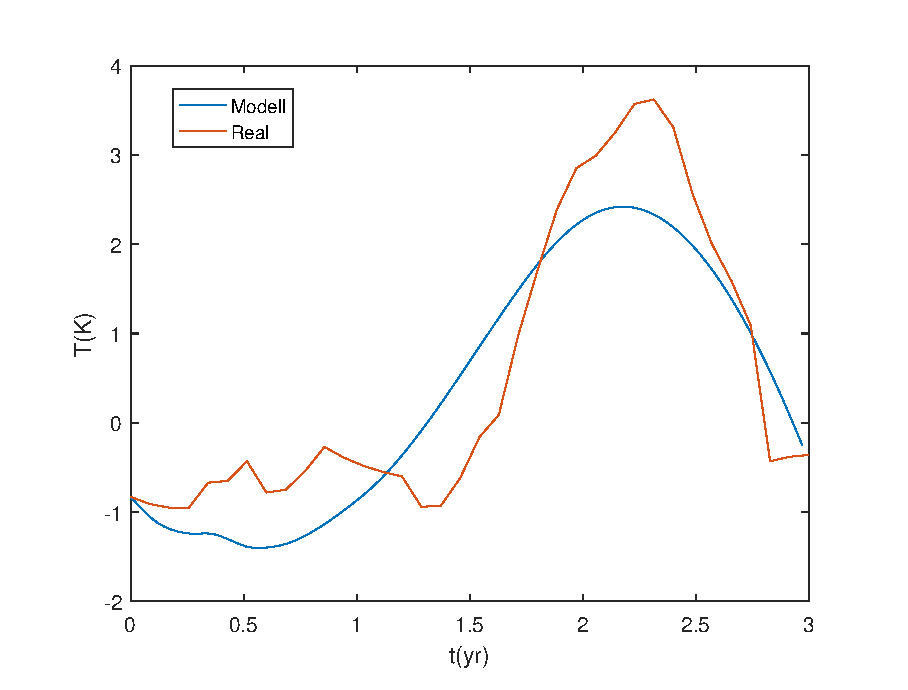
\includegraphics[width=0.66\textwidth,height=0.33\textheight]{verzoegert/inp/figures/sim_3.eps}
	\caption{El-Niño Simulation von 1995-1998 und Vergleich mit realen Daten}
	\label{fig:sim3}
\end{figure}
\begin{figure}
	\centering
	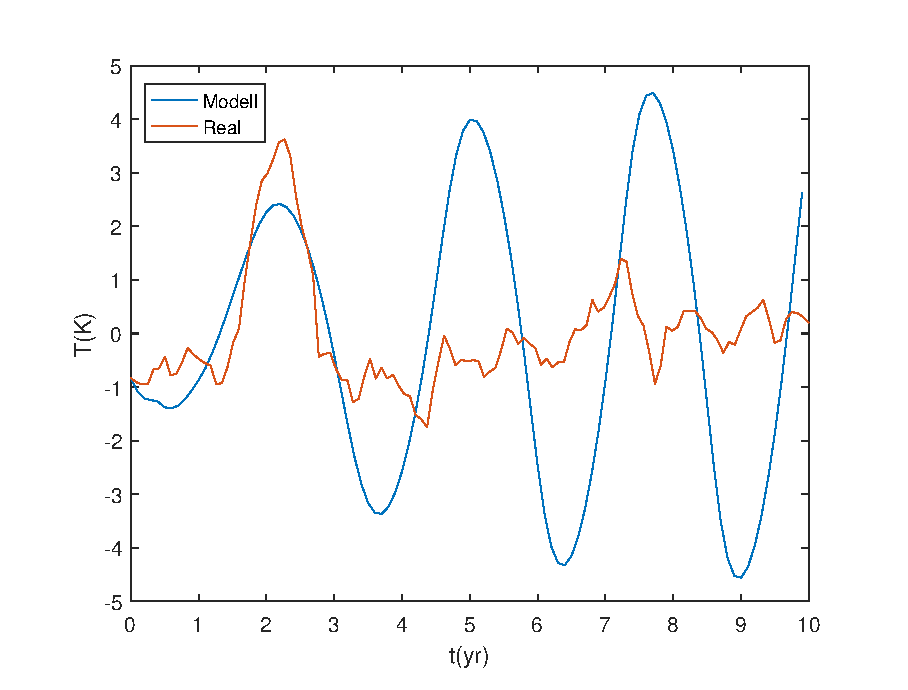
\includegraphics[width=0.66\textwidth,height=0.33\textheight]{verzoegert/inp/figures/sim_10.eps}
	\caption{El-Niño Simulation von 1995-2005 und Vergleich mit realen Daten}
	\label{fig:sim10}
\end{figure}
Mit den richtigen Konstanten lassen sich für kurze Zeiten relativ gute Vorhersagen machen.
Allerdings ist das El-Niño-Phänomen (vgl. Abbildung \ref{fig:elnino}) extrem unkonstant und bräuchte ein komplexeres Modell.
Über längere Zeit versagt das Modell, da es immer zu einer gleichmäßigen Oszillation kommt.

Interessant ist, dass die DDE das kurzfristige Verhalten (1 Jahr, Abbildung \ref{fig:sim1}) richtig berechnet.
Das sieht man an der kurzen Richtungsänderung zwischen 0,3 und 0,4 Jahren.



\subsection{Fazit}
Mit verzögerten Differentialgleichungen können diverse Probleme gelöst werden.
DDEs können analytisch untersucht werden, die Komplexität nimmt allerdings schnell zu.
Eine numerische Simulation ist daher zwingend.
Eine solche Simulation kann relativ einfach erstellt werden und liefert gute Resultate.
Man sollte die Resultate trotzdem genau prüfen, da die Lösungen schnell instabil werden können (vgl. \ref{num:instabil}).

Das Modell zur Modellierung des El-Niño-Phänomens ist sicher noch nicht vollständig.
Es ist aber ein schönes Beispiel einer Anwendung von verzögerten Differentialgleichungen. 

\printbibliography[heading=subbibliography]
\end{refsection}
